\chapter{Probability and Math Revision}
\label{ap:revision-probability}

\section{Random variable}
We call random variable X a measurable real-valued  function of possible outcomes ($\Omega$ ) defined on a sample space($E$).

\begin{equation}
	X: \Omega \rightarrow E
\end{equation}

\section{Probability Density Function (PDF)}

Let X be a continuous random variable. We say that X is a continuous random variable if there is a function $f (x) $, that satisfies for a set $B = \{b \in \mathbb{R} | b_ {1} \leq b \leq b_ {2}\} $, defined for all $x = \{x \in \mathbb{R}| - \infty \leq x \leq + \infty\} $, having the property: 

\begin{equation}
	P(X \in B) = \int_{b_{1}}^{b_{2}}f(x) dx 
\end{equation}

Where $P$ is the probability function of the random variable $x$. $f(x)$ is called probability density function of the random variable $X$\cite{ross-probability}. 

\section{Cumulative Distribution Function (CDF)}

The Cumulative Distribution Function of a random variable $X$, we represent by $F (x) $ is defined at a given point $\ \in X$ as\cite{ross-probability}: 

\begin{equation}
F(a) = P(X \leq a) = \int_{- \infty}^{a}f(x) dx 
\end{equation}

\section{Expected value, Mean, Variance and Standard Deviation}

Let $X$ be a constinuous random variable, and $f(x)$ be its  density function f (x). Then the expected value of $X$ is defined by:

\begin{equation}
E[X] =  \int_{- \infty}^{+ \infty}xf(x) dx 
\end{equation}

For a random variable normally distributed $X_{normal}$ the result of this definition is equals to the mean $\mu$ of the distribution($E[X_{normal}] = \mu$). For an exponential distribution is equals to the inverse of its rate($E[X_{exponential}] = 1/\lambda$).


The variance of a random variable $X$, denoted by $Var(X)$, is defined by:

\begin{equation}
Var(X) =  E[( X - E[x])^{2}] 
\end{equation}


For a random variable $X$ normally distributed, the variance is equal to its standard deviation ($Var(X) = \sigma^{2}$)\cite{ross-probability}. 


% For a normal distribution the result of this definition is  its mean ($E[X_{normal}] = \mu$), and for an exponential distribution is equals to the inverse of its rate:  ($E[X_{exponential}] = \frac{1}{\lambda}$).


\section{Stochastic Process}

A stochastic process of a random variable represented by $\{X(t)| t \in T\}$ is a collection of random variables. Since $t$ is often interpreted as time, $X (t) $ is usually referred as the state of the process at a given time $t$\cite{ross-probability}.


\section{Self-similarity}

A self similar object has the property of looking "roughly" the same at any scale. Self-similar objects are described by the power law:

\begin{equation}
	N = s^{d}
\end{equation}

where 
\begin{equation}
	d = \frac{\ln{N}}{\ln{s}}
\end{equation}

is the dimension of the scaling law, called  Hausdorff dimension\cite{web-self-similar}. 


\begin{figure*}[ht!]
	\centering
	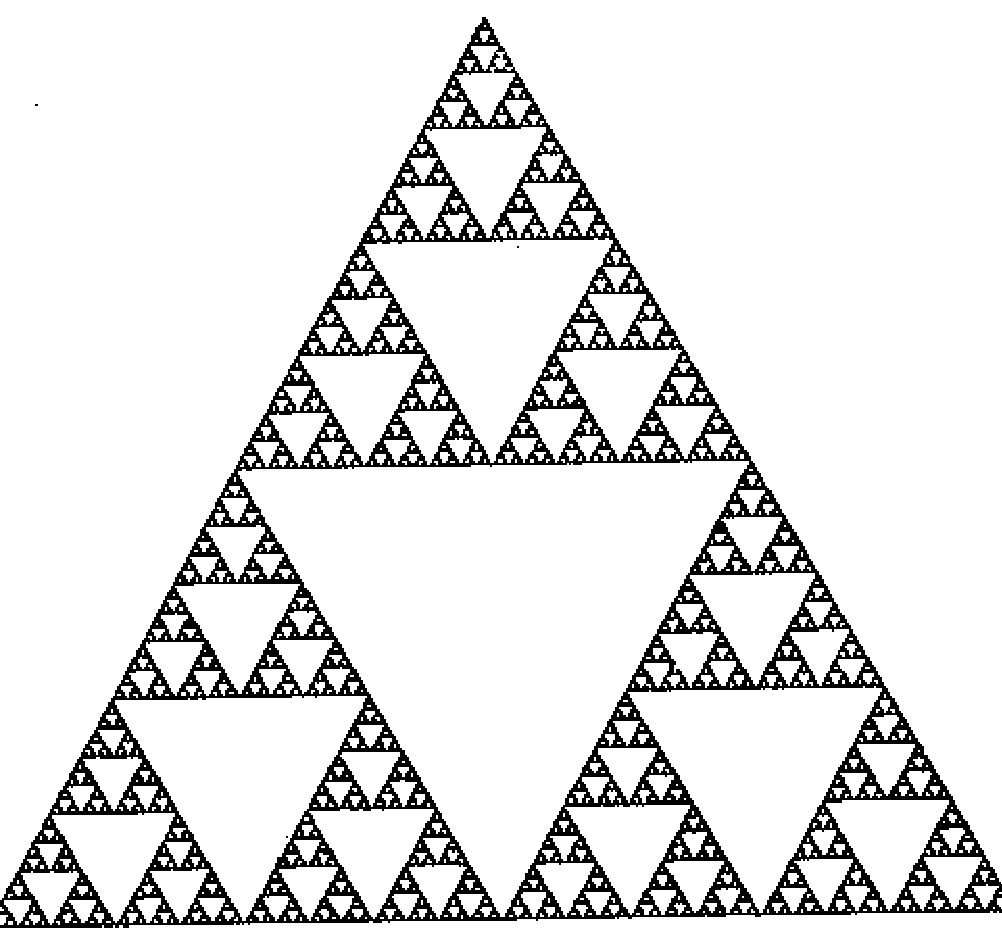
\includegraphics[height=2.0in]{figures/apA/tritrans}
	\caption{This is a classical example of a self-similar figure, caled Sierpinski triangle.}
	\label{fig:self-similar-figure-example}
\end{figure*}


\section{Heavy-tailed distributions}

Heavy tailed distributions are probability distributions whose tails are not exponentially bounded.  A distribution of of a random variable $X$, with cumulative distribution F(x), is said to be heavy tailed, if it satisfies this condition for all $\lambda \in \mathbb{R}$:

\begin{equation}
	\lim_{x\to\infty} e^{\lambda x} (1 - F(x)) = \infty
\end{equation}

%\section{Hurst Exponent}
% se der tempo eu faço isso... é mt nadaver

\section{Akaike information criterion (AIC) and Bayesian information criterion (BIC)}

Suppose that we have an statistical model $M$ of some dataset ${\boldsymbol{x} = \{x_1, ..., x_n}\}$, with $n$ independent and identically distributed observations of a random variable $X$. This model can be expressed by a PDF $f(x| \boldsymbol{\theta})$, where $\boldsymbol{\theta}$ a vector of parameter of the PDF, $\boldsymbol{\theta} \in \mathbb{R}^{k}$ ($k$ is the number of parameters). The  likelihood function  of this model $M$ is given by:

\begin{equation}
L(\boldsymbol{\theta}|\boldsymbol{x} ) =  f(x_1|\boldsymbol{\theta})\cdot...\cdot f(x_n|\boldsymbol{\theta}) = \prod_{i = 1}^{n}f(x_i|\boldsymbol{\theta})
\end{equation}

Now, suppose we are trying to estimate the best statistical model, from a set ${M_1, ..., M_n}$, each one whit an estimated vector of parameters  ${\boldsymbol{\hat{\theta_1}}}, ..., {\boldsymbol{\hat{\theta_n}}}$. $AIC$ and $BIC$ are defined by:

\begin{equation}
AIC = 2k - \ln(L(\boldsymbol{\hat{\theta}}|\boldsymbol{x}))
\end{equation}

\begin{equation}
BIC = k\ln(n) - \ln(L(\boldsymbol{\hat{\theta}}|\boldsymbol{x}))
\end{equation}

In both cases, the preferred model $M_i$, is the one with the smaller value of $AIC_i$ or $BIC_i$.


\section{Gradient Descendent Algorithm}

Given a linear hypothesis for a dataset:

\begin{equation}
	\boldsymbol{h_{\theta}} = \boldsymbol{\theta}^{T}\boldsymbol{x} 
\end{equation}

were $\boldsymbol{h_{\theta}}, \boldsymbol{\theta}, \boldsymbol{x} \in \mathbb{R}^{m}$. If $m = 2$ we will just have a simple linear equation $h_{\theta}(x) = \theta_{0} + \theta_{1}x$.

The goal of the gradient descendent is to minimize the cost function, defined by:

\begin{equation}
	J(\boldsymbol{\theta}) = \frac{1}{2m} \sum_{i = 1}^{m}  ( \boldsymbol{h_{\theta}}(x^{(i)} - y^{(i)} )^{2}
\end{equation}




To do this, we initialize a $\boldsymbol{\theta_{j}}$ vector (usually with zeros), and repeat this procedure, until $\boldsymbol{\theta_{j}}$ converges:

\begin{equation}
	\boldsymbol{\theta_{j + 1}} := \boldsymbol{\theta_{j}} - \alpha \frac{1}{m} \sum_{i = 1}^{m}  ( \boldsymbol{h_{\theta}}(x^{(i)} - y^{(i)} )x_{j}^{i}
\end{equation}

where $\alpha$ is the step value, typically a small positive number. All values of $\boldsymbol{\theta_{j}}$ must be updated simultaneously. 

